\documentclass[12pt]{article}
\setlength{\oddsidemargin}{0in}
\setlength{\evensidemargin}{0in}
\setlength{\textwidth}{6.5in}
\setlength{\parindent}{0in}
\setlength{\parskip}{\baselineskip}

\usepackage{amsmath,amsfonts,amssymb,bm,graphics,pgfplots,framed,dsfont}
\usepackage[scale=0.75,top=1cm,bottom=3cm]{geometry}

\begin{document}

\textbf{Minh Anh Nguyen }\\
\textbf{Calculus 1 Assignment-11}\\
\textbf{Section: 04}\\
\textbf{TA's name: Arthur Huey}

\hrulefill

Section 4.3:

\begin{enumerate}
\setcounter{enumi}{1}
    \item Let $g(x) = \int_{0}^{x} f(t)dt$, where $f$ is the function whose graph is shown.
    \begin{center}
        \includegraphics{./img/img-0.png}        
    \end{center}
    \begin{enumerate}
        \item Evaluate $g(x)$ for $x = 0,1,2,3,4,5,6$.
        \begin{align*}
        g(0) &= 0\\
        g(1) &= 0.5\\
        g(2) &= 0\\
        g(3) &= -0.5\\
        g(4) &= 0\\
        g(5) &= 1.5\\
        g(6) &= 2.5
        \end{align*}
        \item Estimate $g(7)$.
        \[g(7) = 4.375\]
        \item Where does $g$ have a maximum value? Where does it have a minimum value?\\
        The function g has a maximum value at x = 7 and minimum value at x = 3.
        \item Sketch a rough graph of g.
        \begin{center}
            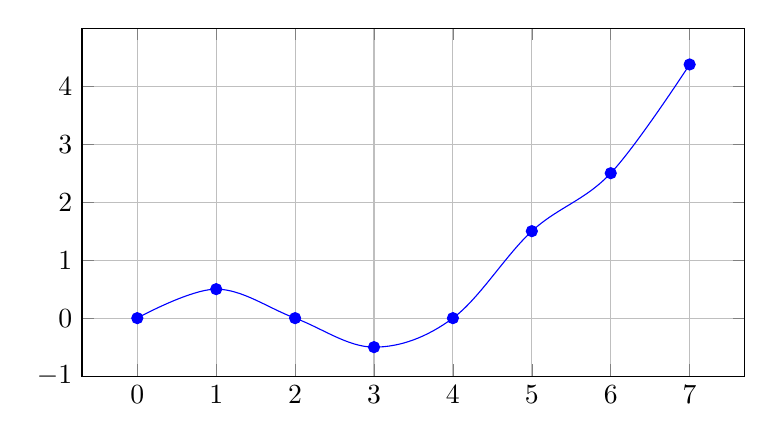
\begin{tikzpicture}
                \begin{axis}[
                    width=10cm, height=6cm,
                    grid=major,
                    ymin=-1, ymax=5,
                    smooth,
                    tension=0.6,
                    ytick={-1,0,1,2,3,4},
                    xtick={0,1,2,3,4,5,6,7},
                    ylabel style={rotate=-90}
                ]
                
                % Plotting the points with smooth curve
                \addplot[
                    color=blue,
                    mark=*,
                    mark options={fill=blue},
                    smooth,
                    tension=0.6
                ]
                coordinates {(0,0) (1,0.5) (2,0) (3,-0.5) (4,0) (5,1.5) (6,2.5) (7,4.375)};
                \end{axis}
                \end{tikzpicture}
        \end{center}
    \end{enumerate}
\newpage
\setcounter{enumi}{5}
    \item The graph of a function $f$ is shown. Let $g$ be the function that represents the area under the graph of $f$ between 0 and $x$.
    \begin{center}
        \includegraphics{img/img-1.png}
    \end{center}
    \begin{enumerate}
        \item Use geometry to find a formula for $g(x)$.
        \[g(x) = \frac{3x^2}{2}\]
        \item Verify that $g$ is an antiderivative of $f$ and explain how this confirms Part 1 of the Fundamental Theorem of Calculus for the function $f$.
        \[g'(x) = (\frac{3x^2}{2})'= 3x = f(x)\]
        Because g(x) is both continuous and differentiable everywhere, g'(x) = f(x) confirms Part 1 of the Fundamental Theorem of Calculus.
    \end{enumerate}
    \item Sketch the area represented by g(x). Then find g'(x) in two ways:
    \[g(x) = \int_{1}^{x} t^2dt\]
    \begin{enumerate}
        \item by using Part 1 of the Fundamental Theorem and
        \[g(x) = \int_{1}^{x} t^2dt \text{, where} f(t) = t^2\]
        Hence, $g'(x) = f(x) = x^2$.
        \item by evaluating the integral using Part 2 and then differentiating.
        \[g(x) = \int_{1}^{x} x^2 = (\frac{x^3}{3} + C)|_1^x = \frac{x^3}{3} - \frac{1}{3}\]
        \[g'(x) = (\frac{x^3}{3} - \frac{1}{3})' = x^2\]
        \begin{center}
            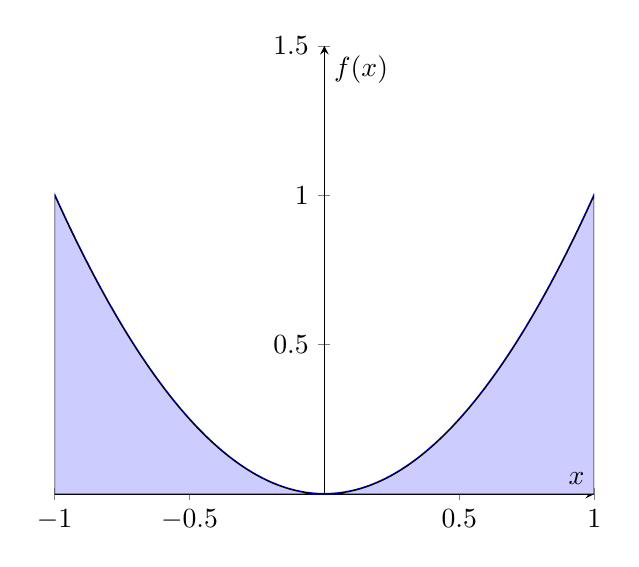
\begin{tikzpicture}
            \begin{axis}[
                axis lines = middle,
                xlabel = {$x$},
                ylabel = {$f(x)$},
                ymin = 0, ymax = 1.5,
                xmin = -1, xmax = 1,
                samples = 100,
                domain = -1.5:1.5,
            ]
                % Plot f(x) = x^2
                \addplot[blue, thick] {x^2};
    
                % Fill the area under f(x) from x = -1 to x = 1
                \addplot[
                fill=blue!20,
                domain=-1:1
                ] {x^2} \closedcycle;
            \end{axis}
            \end{tikzpicture}    
        \end{center}
    \end{enumerate}
\setcounter{enumi}{8}
    \item Use Part 1 of the Fundamental Theorem of Calculus to find the derivative of the function.
    \[g(x) = \int_{0}^{x} \sqrt{t + t^3}dt\]
    Due to Part 1 of the Fundamental Theorem of Calculus:
    \[g'(x) = \sqrt{x+x^3}\]
\setcounter{enumi}{13}
    \item Use Part 1 of the Fundamental Theorem of Calculus to find the derivative of the function.
    \[R(y) = \int_{y}^{2} t^3 \sin (t) dt = -\int_{2}^{y} t^3 \sin (t) dt = \int_{2}^{y} - t^3 \sin (t) dt\]
    Due to Part 1 of the Fundamental Theorem of Calculus:
    \[R'(y) = - t^3 \sin (t)\]
\setcounter{enumi}{21}
    \item Use Part 2 of the Fundamental Theorem of Calculus to evaluate the integral and interpret the result as an area or a difference of areas. Illustrate with a sketch.
    \[\int_{0}^{4} (x^2-4x)dx\]
    Let F be the antiderivative of the function $f(x) = x^2 - 4x$.
    \[F(x) = \frac{x^3}{3} - 2x^2 + C\]
    \[\int_{0}^{4} (x^2-4x)dx = F(4) - F(0) = (\frac{x^3}{3} - 2x^2)|^4_0 = \frac{4^3}{3} - 2(4)^2 - 0 = -\frac{32}{3}\]
    \begin{center}
    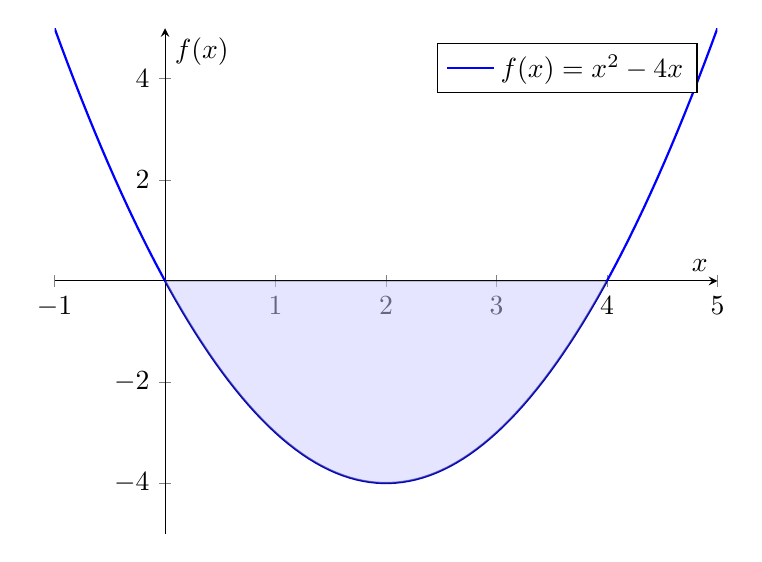
\begin{tikzpicture}
        \begin{axis}[
            axis lines = middle,
            xlabel = $x$,
            ylabel = {$f(x)$},
            ymin = -5, ymax = 5,
            xmin = -1, xmax = 5,
            samples = 100,
            domain = -1:5,
            width=10cm,
            height=8cm,
            legend pos = north east,
        ]
            % Plot the function
            \addplot[blue, thick] {x^2 - 4*x};
            \addlegendentry{$f(x) = x^2 - 4x$}
            
            % Shade the area under the curve from x=0 to x=4
            \addplot [
                domain=0:4, 
                samples=100, 
                fill=blue!20, 
                opacity=0.5
            ] {x^2 - 4*x} \closedcycle;
        \end{axis}
    \end{tikzpicture}
    \end{center}
\setcounter{enumi}{26}
    \item Evaluate the integral
    \[\int_{0}^{2} (\frac{4}{5}t^3 - \frac{3}{4}t^2 + \frac{2}{5}t)dt = (\frac{1}{5}t^4 - \frac{1}{4}t^3 + \frac{1}{5}t^2)|_{0}^{2}\]
    \[ = \frac{1}{5}(2)^4 - \frac{1}{4}(2)^3 + \frac{1}{5}(2)^2 - 0 = 2\]
\setcounter{enumi}{34}
    \item Evaluate the integral
    \[\int_{0}^{1} (u+2)(u-3)du = \int_{0}^{1} (u^2 - u -6) du = (\frac{u^3}{3} - \frac{u^2}{2} - 6u)|^{1}_{0}\]
    \[ = \frac{1^3}{3} - \frac{1^2}{2} - 6(1) - 0 = -\frac{37}{6}\]
\setcounter{enumi}{44}
    \item Evaluate the integral
    \[\int_{0}^{\pi} f(x) \, dx \quad \text{where} \quad f(x) = 
    \begin{cases} 
    \sin x & \text{if } 0 \leq x < \frac{\pi}{2} \\
    \cos x & \text{if } \frac{\pi}{2} \leq x \leq \pi 
    \end{cases}
    \]
    \[ = \int_{0}^{\pi/2} f(x) dx + \int_{\pi/2}^{\pi} f(x) dx = \int_{0}^{\pi/2} \sin x dx + \int_{\pi/2}^{\pi} \cos x dx\]
    \[ = (-\cos x)|^{\pi/2}_{0} + (\sin x)|^{\pi}_{\pi/2} = (-\cos \pi/2 + \cos 0) + (\sin \pi - \sin \pi/2) = 1-1 = 0\]
\setcounter{enumi}{46}
    \item Sketch the region enclosed by the given curves and calculate its area.
    \[y = \sqrt{x}, y = 0, x = 4\]
    \begin{center}
        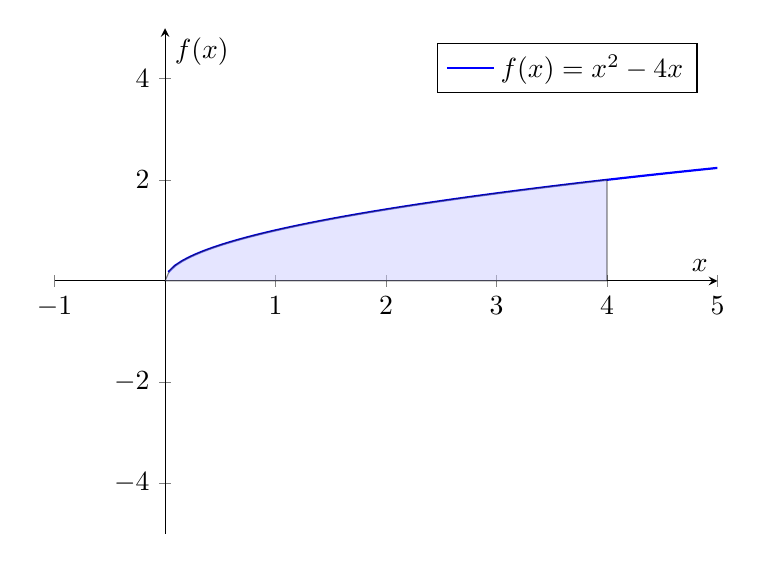
\begin{tikzpicture}
            \begin{axis}[
                axis lines = middle,
                xlabel = $x$,
                ylabel = {$f(x)$},
                ymin = -5, ymax = 5,
                xmin = -1, xmax = 5,
                samples = 100,
                domain = -1:5,
                width=10cm,
                height=8cm,
                legend pos = north east,
            ]
                % Plot the function
                \addplot[blue, thick] {sqrt(x)};
                \addlegendentry{$f(x) = x^2 - 4x$}
                
                % Shade the area under the curve from x=0 to x=4
                \addplot [
                    domain=0:4, 
                    samples=100, 
                    fill=blue!20, 
                    opacity=0.5
                ] {sqrt(x)} \closedcycle;
            \end{axis}
        \end{tikzpicture}    
    \end{center}
    If y = 0, x = 0. Hence, the region enclosed by x = 0 and x = 4, and the arae of the region is $\int_{0}^{4} \sqrt{x}$.
    \[\int_{0}^{4} \sqrt{x} = (\frac{2x^{3/2}}{3})|^{4}_{0} = \frac{2(4)^{3/2}}{3} - 0 = \frac{16}{3}\]
\setcounter{enumi}{54}
    \item What is wrong with the equation?
    \[\int_{-2}^{1} x^{-4}dx = (\frac{x^{-3}}{-3})|^{1}_{-2} = -\frac{3}{8} \]
    Because the function $x^{-4}$ is not continuous at x = 0. Hence, the integral is undefined.
\setcounter{enumi}{59}
    \item Find the derivative of the function
    \[g(x) = \int_{1-2x}^{1+2x} t \sin t dt\]
    Using the Leibniz rule:
    \[g'(x) = ((1+2x)\sin (1+2x))(1+2x)' - ((1-2x)\sin (1-2x))(1-2x)' \]
    \[ = 2((1+2x)\sin (1+2x)) + 2((1-2x)\sin (1-2x)) \]
\setcounter{enumi}{66}
    \item If $f(1) = 12$, $f'$ is continuous, and $\int_{1}^{4} f'(x)dx = 17$, what is the value of $f(4)$?
    \[\int_{1}^{4} f'(x)dx = f(4) - f(1) = 17\]
    \[f(4) - 12 = 17\]
    \[f(4) = 29\]
\setcounter{enumi}{73}
    \item Evaluate the limit by first recognizing the sum as a Riemann sum for a function defined on [0,1].
    \[\lim_{n \to \infty} \frac{1}{n} (\sqrt{\frac{1}{n}} + \sqrt{\frac{2}{n}} + \sqrt{\frac{3}{n}} + ... + \sqrt{\frac{n}{n}})\]
    \[ = \lim_{n \to \infty} \frac{1}{n} (\frac{\sqrt{1} + \sqrt{2} + \sqrt{3} + ... + \sqrt{n}}{\sqrt{n}})\]
    \[ = \lim_{n \to \infty} \Sigma^{n}_{i = 1} \frac{1}{n} (\frac{\sqrt{i}}{\sqrt{n}})\]
    \[ = \lim_{n \to \infty} \Sigma^{n}_{i = 1} \frac{1}{n} (\sqrt{\frac{i}{n}})\]
    \[\Delta x = \frac{1}{n}\]
    \[x_i = \frac{i}{n}\]
    Hence,
    \[a = 0, b = 1\]
    \[f(x) = \sqrt{x}\]
    \[\lim_{n \to \infty} \Sigma^{n}_{i = 1} \frac{1}{n} (\sqrt{\frac{i}{n}}) = \int_{0}^{1} \sqrt{x} dx = (\frac{2x^{3/2}}{3})|_{0}^{1} = \frac{2}{3}\]
\end{enumerate}

\newpage
Section 4.4:
\begin{enumerate}
\setcounter{enumi}{1}
    \item Verify by differentiation that the formula is correct.
    \[\int \tan^2 x dx = \tan x - x + C\]
    \[(\tan x - x + C)' = \sec^2 x  - 1 = \tan^2 x \]
    Hence, the formula is correct.
\setcounter{enumi}{5}
    \item Find the general indefinite integral.
    \[\int (5 + 2 \sqrt{x}) dx = 5x + \frac{4x^{3/2}}{3} + C\]
\setcounter{enumi}{17}
    \item Find the general indefinite integral.
    \[\int \sec t (\sec t + \tan t) dt = \int (\sec^2 t + \sec t \tan t) dt = \tan t + \sec t + C\]
\setcounter{enumi}{32}
    \item Evaluate the definite integral.
    \[\int_{\pi/6}^{\pi/3} (4\sec^2 y) dy = 4 \int_{\pi/6}^{\pi/3} (\sec^2 y) dy = 4 \times (\tan y)|^{\pi/3}_{\pi/6} = 4(\sqrt{3} - \frac{1}{\sqrt{3}}) = 4(\frac{3 - 1}{\sqrt{3}}) = \frac{8}{\sqrt{3}}\]
\setcounter{enumi}{38}
    \item Evaluate the definite integral.
    \[\int_{0}^{\pi/4} \frac{1 + \cos^2 \theta}{\cos^2 \theta} d\theta = \int_{0}^{\pi/4} (\frac{1}{\cos^2 \theta}  + \frac{\cos^2 \theta}{\cos^2 \theta}) d\theta\]
    \[ = \int_{0}^{\pi/4} (\sec^2 \theta  + 1)d\theta = (\tan x + x)|^{\pi/4}_{0} = 1+\pi/4 - 0 - 0 = \frac{4 + \pi}{4}\]
\setcounter{enumi}{42}
    \item Evaluate the definite integral.
    \[\int_{2}^{5} |x - 3| dx\]
    Let $f(x) = |x - 3|$. The function $f(x)$ is negative with $x < 3$ and positive with $x > 3$. \\
    Hence
    \[\int_{2}^{5} |x - 3| dx = -\int_{2}^{3} (x - 3) dx + \int_{3}^{5} (x - 3) dx\]
    \[= -(\frac{x^2}{2}-3x)|^{3}_{2} + (\frac{x^2}{2}-3x)|_{3}^{5} = -(\frac{3^2}{2} - 3(3) - \frac{2^2}{2} + 3(2)) + (\frac{5^2}{2} - 3(5) - \frac{3^2}{2} + 3(3)) = \frac{5}{2}\]
    \[\]

\newpage
\setcounter{enumi}{48}
    \item The area of the region that lies to the right of the y-axis and to the left of the parabola $x = 2y - y^2$ (the shaded region in the figure) is given by the integral $\int_{0}^{2} (2y - y^2)dy$. (Turn your head clockwise and think of the region as lying below the curve $x=2y-y^2$ from $y=0$ to $y=2$.) Find the area of the region.      
    \begin{center}
        \includegraphics{img/img-2.png}
    \end{center}
    The area of the region is:
    \[\int_{0}^{2} (2y - y^2)dy = (y^2 - \frac{y^3}{3})|_{0}^{2} = 2^2 - \frac{2^3}{3} - 0 + 0 = \frac{4}{3}\]
\setcounter{enumi}{50}
    \item If $w'(t)$ is the rate of growth of a child in pounds per year, what does $\int_{5}^{10} w'(t)dt$ represent?\\
    It represents the change of the child's weight between the age of 5 with the age of 10.
    \item The current in a wire is defined as the derivative of the charge: $I(t) = Q'(t)$. (See Example 2.7.3.) What does $\int_{a}^{b} I(t)dt$ represent?\\
    This represents the total change of the current flowing through the wire between time a to b.
\setcounter{enumi}{62}
    \item The acceleration function (in $m/s^2$) and the initial velocity are given for a particle moving along a line. Find
    \[a(t) = t + 4, v(0) = 5, 0 \leq t \leq 10\]
    \begin{enumerate}
        \item the velocity at time $t$ and
        \[v(t) = \int (t + 4) dt = \frac{t^2}{2} + 4t + C\]
        Because $v(0) = 5$:
        \[v(0) = \frac{(0)^2}{2} + 4(0) + C = 5\]
        \[C = 5\]
        Hence, the velocity at time $t$ is:
        \[v(t) = \frac{t^2}{2} + 4t + 5\]
        \item the distance traveled during the given time integral,\\
        The distance traveled during the given time is:
        \[D = \int_{0}^{10} v(t)dt = \int_{0}^{10} (\frac{t^2}{2} + 4t + 5) dt = (\frac{t^3}{6} + 2t^2 + 5t)|_{0}^{10}\]
        \[ = \frac{10^3}{6} + 2(10)^2 + 5(10) - 0 = \frac{1250}{3}\]
    \end{enumerate}
\end{enumerate}

\newpage 
Section 4.5:

\begin{enumerate}
\setcounter{enumi}{2}
    \item Evaluate the integral by making the given substitution.
    \[\int x(2x^2 + 3)^4 dx, u = 2x^2 + 3\]
    \[du = 4x dx\]
    \[\frac{du}{4} = x dx\]
    Hence,
    \[\int x(2x^2 + 3)^4dx = \frac{1}{4}\int u^4 du = \frac{u^5}{20} + C = \frac{(2x^2 + 3)^5}{20} + C\]
    \item Evaluate the integral by making the given substitution.
    \[\int \sin^2 \theta \cos \theta d\theta, u = \sin \theta\]
    \[du = \cos \theta d\theta\]
    Hence, 
    \[\int \sin^2 \theta \cos \theta d\theta = \int u^2 du = \frac{u^3}{3} + C = \frac{(\sin x)^3}{3} + C\]
\setcounter{enumi}{8}
    \item Evaluate the indefinite integral.
    \[\int x \sqrt{1-x^2}dx\]
    Let:
    \[u = 1 - x^2\]
    \[du =- 2xdx\]
    \[-\frac{du}{2} = xdx\]
    Hence:
    \[\int x \sqrt{1-x^2}dx = -\frac{1}{2}\int \sqrt{u}du = -\frac{1}{2} \frac{2u^{3/2}}{3} + C = -\frac{u^{3/2}}{3} + C = -\frac{(1-x^2)^{3/2}}{3} + C\]
\setcounter{enumi}{14}
    \item Evaluate the indefinite integral.
    \[\int \sec 3t \tan 3t dt\]
    Let:
    \[u = 3t\]
    \[du = 3dx\]
    \[\frac{du}{3} = dx\]
    Hence:
    \[\int \sec 3t \tan 3t dt = \frac{1}{3} \int \sec u \tan u du = \frac{\sec u}{3} + C = \frac{\sec 3t}{3} + C \]
\setcounter{enumi}{19}
    \item Evaluate the indefinite integral.
    \[\int \sin x \sin (\cos x) dx\]
    Let:
    \[u = \cos x\]
    \[du = - \sin x dx\]
    \[-du = \sin x dx\]
    Hence:
    \[\int \sin x \sin (\cos x) dx = - \int \sin u du = - (-\cos u) + C = \cos u + C = \cos (\cos x) + C\]
\setcounter{enumi}{23}
    \item Evaluate the indefinite integral.
    \[\int \frac{\sec^2 x}{\tan^2 x}dx\]
    Let:
    \[u = \tan^2 x\]
    \[du = \sec^2x dx\]
    Hence: 
    \[\int \frac{\sec^2 x}{\tan^2 x}dx = \int \frac{1}{u} du = len{|u|} + C = len{|\tan^2 x|} + C\]
\setcounter{enumi}{41}
    \item Evaluate the definite integral.
    \[\int_{1}^{4} \frac{\sqrt{2+\sqrt{x}}}{\sqrt{x}}\]
    Let:
    \[u = \sqrt{x}\]
    \[du = \frac{1}{2\sqrt{x}}dx\]
    \[2du = \frac{1}{\sqrt{x}}dx\]
    Hence:
    \[\int_{1}^{4} \frac{\sqrt{2+\sqrt{x}}}{\sqrt{x}} = 2\int_{1}^{2} \sqrt{2 + u}du\]
    Let:
    \[t = 2 + u\]
    \[dt = du\]
    Hence:
    \[2\int_{1}^{2} \sqrt{2 + u}du = 2\int_{3}^{4} \sqrt{t}dt = 2 \times (\frac{2t^{3/2}}{3})|^{4}_{3} = 2 \times (\frac{2(4)^{3/2}}{3} - \frac{2(3)^{3/2}}{3})\]
\setcounter{enumi}{47}
    \item Evaluate the definite integral.
    \[\int_{-\pi/3}^{\pi/3} x^4 \sin x dx\]
    Because $(-x)^4 = x^4$ and $\sin (-x) = - \sin (x)$.\\
    Hence, their multiply will be an odd function and:
    \[\int_{-\pi/3}^{\pi/3} x^4 \sin x dx = 0\]
\setcounter{enumi}{54}
    \item Evaluate $\int_{-2}^{2} (x+3)\sqrt{4-x^2}$ by writing it as a sum of two integrals and interpreting one of those integrals in terms of an area.
    \[\int_{-2}^{2} (x+3)\sqrt{4-x^2} = \int_{-2}^{2} x\sqrt{4-x^2} + \int_{-2}^{2} 3\sqrt{4-x^2}\]
    Because $- (x\sqrt{4-x^2}) = (-x)\sqrt{4-(-x)^2}$, the function $x\sqrt{4-x^2}$ is a odd function.\\
    Hence, 
    \[\int_{-2}^{2} x\sqrt{4-x^2} = 0\]
    Because $3\sqrt{4-x^2} = 3\sqrt{4-(-x)^2}$, the function $3\sqrt{4-x^2}$ is an even function.\\
    Hence, 
    \[\int_{-2}^{2} 3\sqrt{4-x^2} = 2\int_{0}^{2} 3\sqrt{4-x^2} = 6\int_{0}^{2} \sqrt{4-x^2}\]
    The definite integral $\int_{0}^{2} \sqrt{4-x^2}$ is one fourth of a circle with a radius of 2.\\
    Hence,
    \[6\int_{0}^{2} \sqrt{4-x^2} = 6 \times \frac{1}{4}(\pi 2^2) = 6\pi\]
    Therefore,
    \[\int_{-2}^{2} x\sqrt{4-x^2} + \int_{-2}^{2} 3\sqrt{4-x^2} = 0 + 6\pi = 6\pi\] 
\newpage
\setcounter{enumi}{58}
    \item If $f$ is continuous and $\int_{0}^{4} f(x)dx = 10$, find $\int_{0}^{2} f(2x) dx$.\\
    Let:
    \[u = 2x\]
    \[du = 2dx\]
    \[\frac{du}{2} = dx\]
    Hence,
    \[\int_{0}^{2} f(2x) dx = \frac{1}{2}\int_{0}^{4} f(u) du = \frac{1}{2}10 = 5\]
\setcounter{enumi}{68}
    \item Evaluate the integral.
    \[\int \frac{(ln x)^2}{x} dx\]
    Let
    \[u = ln x\]
    \[du = \frac{1}{x}dx\]
    Hence,
    \[\int \frac{(ln x)^2}{x} dx = \int u^2 du = \frac{u^3}{3} + C = \frac{(ln x)^3}{3} + C\]
\setcounter{enumi}{79}
    \item Evaluate the integral.
    \[\int \frac{x}{1+x^4}dx\]
    Let
    \[u = x^2\]
    \[du = 2xdx\]
    \[\frac{du}{2} = xdx\]
    Hence, 
    \[\int \frac{x}{1+x^4}dx = \frac{1}{2} \int \frac{1}{1 + u^2} du = \frac{\tan^{-1} u }{2} + C = \frac{\tan^{-1} (x^2) }{2} + C\]
\end{enumerate}
\end{document}